%
% LaTeX template for Dual Degree / Masters thesis at IITB
%
% Created by Neehar Jathar
%
% The official requirement has been persisted with, even if some things could look better some other way.
% Tamper with any of the settings as you see fit and, more importantly, as your guide sees fit.
% Most sections have comments. A lot of stuff is explained in Chapter 1 regarding how to use this template.
% Code snippets for inserting figures, tables and equations are also there in Chapter 1
% Hopefully, this will make report making a little easier.
%

% OK. Here goes.

% Preamble

% Official font size is 12. I thought 11 looked better.
% A4 paper size
% Template for one sided printing of the thesis
\documentclass[12pt, a4paper, oneside]{book}


% Set of packages included. These are all the packages I required, maybe some would be unnecessary and some might be missing. 
% Add any new packages you use over here.

\usepackage[utf8]{inputenc}
\usepackage{setspace}
\usepackage{amsmath,amsfonts,amssymb,amscd,amsthm,xspace}
\usepackage{titlesec}
\usepackage{vmargin}
\usepackage{fancyhdr}
\usepackage{caption}
\usepackage{subcaption}
\usepackage{multirow}
\usepackage{multicol}
\usepackage{url}
\usepackage{tabularx}
\usepackage{float}
\usepackage{graphicx}
\usepackage{epstopdf}
\usepackage{booktabs}
\usepackage{rotating}
\usepackage{listings}
%\usepackage[centerlast,small,sc]{caption}
\usepackage[square, numbers, comma, sort&compress]{natbib} % Standard reference style with [3], [4] type numbers in the text and entries sorted according to order of appearance in the References
\usepackage[pdfpagemode={UseOutlines},bookmarks=true,bookmarksopen=true,bookmarksopenlevel=0,bookmarksnumbered=true,hypertexnames=false,colorlinks,linkcolor={black},citecolor={black},urlcolor={black},pdfstartview={FitV},unicode,breaklinks=true]{hyperref}
\hypersetup{urlcolor=black, colorlinks=true} % colors hyperlinks in blue - change to black if annoying

% Math operator definition - may not be required
% If any new operators are required, defien them here
\DeclareMathOperator*{\argmin}{argmin}
\title{\thesisTitle}
\author{\authorName}
\date{\today}

% Currently chapter title has been centered, to left align the chapter title and number, change \centering to \flushleft
\titleformat{\chapter}[display]
  {\normalfont\huge\bfseries\flushleft}
  {\chaptertitlename\ \thechapter}{18pt}{\Huge}

\setmarginsrb   { 3.0cm}  % left margin
                { 1.5cm}  % top margin
                { 2.0cm}  % right margin
                { 2.2cm}  % bottom margin
                { 0.3cm}  % head height
                { 1.2cm}  % head sep
                { 0.3pt}  % foot height
                { 1.0cm}  % foot sep
%section number dept


% End of the Preamble


% Actual document begins
\begin{document}

\newcommand{\HRule}{\rule{\linewidth}{0.5mm}} % New command to make the lines in the title page

% Import all the variable values from Details.tex
% This file contains all the user specific things that need to be changed such as the thesis title, author name etc. 


\newcommand{\thesisTitle}{Implementation of LDPC Decoder Using AHIR Tool Chain }

\newcommand{\degree}{Master of Technology}

\newcommand{\authorName}{Anurag Gupta}

\newcommand{\rollNo}{153070050}

\newcommand{\dept}{Department of Electrical Engineering}

\newcommand{\college}{Indian Institute of Technology Bombay}

\newcommand{\currentyear}{2017}

\newcommand{\currentmonth}{June}

\newcommand{\supervisorOne}{Prof. Madhav P. Desai}

\newcommand{\supervisorTwo}{Prof. Supervisor Two}

\newcommand{\examinerOne}{Prof. Examiner One}

\newcommand{\examinerTwo}{Prof. Examiner Two}

\newcommand{\chairman}{Prof. Chairman}


% Use roman page numbering style (i, ii, iii, iv...) for the pre-content pages
\frontmatter

% Line spacing of 1.5 as per IIT requirement. If you think it looks too spaced out, use 1.3
% I think 11 pt font with 1.3 spacing looks quite good
\setstretch{1.3}

% Import all the pages in the front matter
% This file contains the templates for the first few pages of the thesis including 
% 1. Title page
% 2. Dedication
% 3. Dissertation approval
% 4. Declaration of authorship
% 5. Abstract


%   1. TITLE
\newcommand{\titlePage}{

% No page number
\thispagestyle{empty}
\begin{center}

% thesis title
\vspace*{15px}
{\Huge\bfseries \thesisTitle}\\[1.0cm] 

% submitted in partial fulfillment etc.
\textit{Submitted in partial fulfillment of the requirements\\[0.2cm] of the degree of\\[0.2cm] \degree}\\[2.0cm]
 
% author
\textit{by}\\[0.2cm]
\authorName \\[0.2cm] (\textit{Roll no.} \rollNo) \\[2.0cm]

% supervisor
\textit{Supervisor:}\\[0.2cm]
% or
% \textit{under the supervision of}\\[0.2cm]
\supervisorOne \\[2.0cm]

% iit-b logo

\includegraphics[width=0.25\textwidth]{Figures/iitb_logo.jpg}

\vspace*{10px}

% department and college
\dept\\[0.2cm]
\college\\[0.2cm]

% year
\currentyear\\[4cm] 

\end{center}

\clearpage
}

%   2. DEDICATION
\newcommand{\dedication}{
\thispagestyle{empty}
\vspace*{75px}
\begin{center}\large{\textit{Dedicated to ...}}\end{center}

\clearpage
}

%   3. DISSERTATION APPROVAL

\newcommand{\approval}{
% if you use a dedication, then use a page number with the plain page style
\thispagestyle{plain}
% else, use no page number with the empty page style
%\thispagestyle{empty}


% page title
\begin{center}{\huge\bf Dissertation Approval\par}\end{center}

\vspace*{15px}

\noindent This dissertation entitled 
% title
\textbf{``\thesisTitle"}, submitted by 
% author
\authorName  
(Roll No.  \rollNo),
is approved for the award of degree of 
% degree
\degree 
in 
% branch
XYZ Engineering.\\[1.0cm]

% examiners and supervisors
\begin{flushright}
\textbf{{Examiners}}\\[0.8cm]
\examinerOne\quad\rule{0.3\textwidth}{.3pt}\\[0.8cm]
\examinerTwo\quad\rule{0.3\textwidth}{.3pt}\\[1.6cm]

\textbf{{Supervisor}}\\[0.8cm]
\supervisorOne \quad\rule{0.3\textwidth}{.3pt}\\[1.6cm]

\textbf{{Chairman}}\\[0.8cm]
\chairman\quad\rule{0.3\textwidth}{.3pt}\\[2.4cm]

\end{flushright}
\textbf{Date:} ...... \currentmonth { } \currentyear\\[0.3cm]
\textbf{Place:}\quad\rule{0.5\textwidth}{.3pt} 

% start a new page
\clearpage
}

%   4. DECLARATION OF AUTHORSHIP
\newcommand{\authorship}{
\thispagestyle{plain}

\begin{center}{\huge\bf Declaration of Authorship\par}\end{center}

\vspace*{15px}

% institute declaration text
\noindent I declare that this written submission represents my ideas in my own words and where others' ideas or words have been included, I have adequately cited and referenced the original sources.  I also declare that I have adhered to all principles of academic honesty and integrity and   have   not   misrepresented   or   fabricated   or   falsified   any   idea/data/fact/source   in   my submission.  I understand that any violation of the above will be cause for disciplinary action by the Institute and can also evoke  penal action from the sources which have thus not been properly cited or from whom proper permission has not been taken when needed.

\vspace*{10px}

% signature
\begin{flushright}
{Signature: ......................................\\[0.4cm]}

% author name
{\textbf{\authorName}\\[0.0cm]\rollNo\\[2.0cm]}

\end{flushright}
% date
\begin{flushleft}
{Date: ...... \currentmonth { } \currentyear\\}
\end{flushleft}


% start a new page
\clearpage 
}

%   5. ABSTRACT
\newcommand{\abstractpage}{
\thispagestyle{plain}

% header-type text for the abstract - optional
\small {\noindent\authorName/ \supervisorOne{ }(Supervisor): \textbf{``\thesisTitle"}, \textit{Dual Degree Dissertation}, \dept, \college, \currentmonth { } \currentyear.}\\[0.0cm]
\HRule\\[0.2cm]


\vspace*{10px}

\begin{center}{\huge{\textit {Abstract}}\par}\end{center}

\vspace*{10px}

% Abstract text - Type abstract here
\noindent Enter Abstract text here, in the file TheFrontMatter.tex \\[0.2cm]

% Index terms
\noindent \textbf{Index terms:} 

% Start a new page
\clearpage 
}


\titlePage

\setcounter{page}{1}
\dedication

\addcontentsline{toc}{chapter}{Dissertation Approval}
\approval

\addcontentsline{toc}{chapter}{Declaration of Authorship}
\authorship

\addcontentsline{toc}{chapter}{Abstract}
\abstractpage

\pagestyle{fancy}

% Set the left side page header to "Contents"
\lhead{\emph{Contents}} 

% Write out the Table of Contents
\tableofcontents 

% Set the left side page header to "List of Figures"
\lhead{\emph{List of Figures}} 

% Write out the List of Figures
\listoffigures 
\addcontentsline{toc}{chapter}{List of Figures}

% Set the left side page header to "List of Tables"
\lhead{\emph{List of Tables}} 

% Write out the List of Tables
\listoftables
\addcontentsline{toc}{chapter}{List of Tables}


\fancyhead{}
\rhead{\thepage}


% Use arabic page numbering style (1, 2, 3...) for the body of the report
\mainmatter

% Import the Chapters
% Introduction

% Main chapter title
\chapter{Introduction} 
% Change X to a consecutive number; for referencing this chapter elsewhere, use \ref{ChapterX}
\label{Chapter1} 
% This is for the header on each page
\lhead{Chapter 1. \emph{Introduction}}


\section{Motivation }
The error performance of the low density parity check  codes approach to Shannon limit, which make low density parity check code the best known codes. An active research is going on to implement the low density parity check decoder for storage devices to achieve the bit error rate of the order of $10^{-16}$. Thus, to make a low density parity check  decoder with a optimum cost and performance trade off is a challenging task.

\section{Organisation of the Report }

In chapter 1, we have discussed the basics of error correction in a communication channel. In chapter 2, we have discussed how to generate different parity check matrices. In chapter 3, we have discussed different decoding algorithms in detail. In chapter 4, we have shown the results of the C level implementation of Min Sum decoding algorithm. In chapter 5, we have discussed the concept and procedure to partition a parity check matrix. Level of parallelism is taken as a metric and results are plotted and discussed. In chapter 6, we have deployed partitioning in the matrix and modified the decoding algorithm to parallelise the hardware. In chapter 7, the conversion of the algorithms from C to VHDL is discussed along with results of the implementation of the algorithm on FPGA.
\section{Basics of Error Correction }
  
The goal of communication is to transmit a message and receive it correctly even after noisy transmission through the channel. This is achieved by introducing redundancy in the message at the transmitter side, called as encoding of message. The encoded message is called codeword. Then codeword is then transmitted through the noisy channel, which alters the codeword. By some error correcting algorithm the message is extracted back at receiver side, called decoding of the codeword. Thus, the error free transmission takes place by applying error correcting codes in communication system.\\
We have a k bit long message. To encode it we introduce m redundant bits (called parity bits) to form an $n(=m+k)$ bit long codeword. This category of codes are called (n,k) block codes. 

\subsection{Parity Check Matrix}

The codeword must satisfy a group of conditions to ensure error free transmission or to indicate the error has taken place. If error occurs, the error can be corrected by applying some algorithm on those group of conditions . The group of conditions are called parity check equations.The matrix form of the condition is called parity check matrix. \\
Example: If a code block $y=[c_1\, c_2\,c_3\, c_4\, c_5\, c_6]$ has to satisfy following parity check equations. 
\begin{align}
c_1 \oplus c_2 \oplus c_4 =0 \\
 c_2 \oplus c_3 \oplus c_5 =0 \\
c_1 \oplus c_2 \oplus c_3 \oplus c_6 =0 
\end{align}  
Then it's parity check matrix is as follows:
\begin{align}
 H= \left[ \begin{array}{cccccc}
1 & 1 & 0 & 1 & 0 & 0\\
0 & 1 & 1 & 0 & 1 & 0\\
1 & 0 & 0 & 0 & 1 & 1\\
0 & 0 & 1 & 1 & 0 & 1  
\end{array} \right]  
\end{align} 
s.t. $Hy^T=0$.

\subsection{Encoding of Message}
We can rewrite the above equations (1),(2),(3) as:
\begin{align}
c_4 = c_1 \oplus c_2 \\
c_5 = c_2 \oplus c_3 \\
c_6 = c_1 \oplus c_2 \oplus c_3  
\end{align}  
We can find parity check bits $c_4,c_5,c_6$ by message bits $c_1,c_2,c_3$.
Thus we can encode message bits to find codeword. \\
Encoding is preferably done in matrix form, by manipulating parity check matrix to find a generator matrix.
If parity check matrix can be written in the form
$H = [A, I_{n- k} ]$,
where A is an $(n-k)$xk binary matrix and $I_{n-k}$ is the identity matrix of order
$(n-k)$. The generator matrix is then
$G = [I_k , A^T ]$.
s.t $GH^T = 0$. \\
\begin{align}
[c_1 c_2 ... c_6]=[c_1 c_2 c_3] \left[ \begin{array}{cccccc}
1 & 0 & 0 & 1 & 0 & 1\\
0 & 1 & 0 & 1 & 1 & 1\\
0 & 0 & 1 & 0 & 1 & 1  
\end{array} \right]
\end{align}
 

Thus, if m is message block containing message bits $[c_1 c_2 c_3]$, then codeword can be generated as $y=mG$.

\subsection{Transmission of the Code Block}
The code block is then transferred through a noisy communication channel that corrupts the code block. According to the behaviour of the noise that is added to the code block, various models of communication channels exists. 
\subsubsection{Binary Symmetric Channel}
 As the name suggests the channel is binary, it has two input symbols and two output symbols. The channel is symmetric because the probability of receiving 0 when 1 was send is same as probability of receiving 1 when 0 was sent. The error probability is also called cross over probability. The transition probability diagram is shown in figure \ref{bsc}
 \begin{figure}[h]
\centering
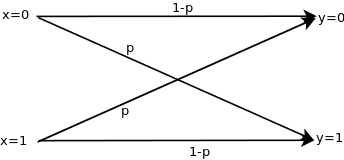
\includegraphics[height=6cm,width=12cm]{bsc}
\caption[Transition probability diagram of Binary Symmetric Channel]{Binary Symmetric Channel}
\label{bsc}
\end{figure}
The cross over probability is denoted as p.
\begin{align} p(y=0|x=1) = p(y=1|x=0) = p  \end{align}
\begin{align} p(y=1|x=1) = p(y=0|x=0) = 1-p  \end{align}
\subsubsection{AWGN (A White Gaussian Noise Channel)}
If a signal in a digital system is represented a continuous random variable as,
\begin{align} Y = X + Z \end{align}
where X is the digital information carrier and Z is the noise component then we can define a Gaussian channel that has input X and output Y, with noise as a Gaussian random variable Z. \\
The pdf of a Gaussian random variable is expressed as follows: \\
\begin{align} f_y(x) = \dfrac{1}{\sqrt{2\pi\sigma^{2}}} \exp{\dfrac{-(x-m)^2}{2\sigma^2}}
 \end{align} 
where m is mean and sigma is standard deviation of the random variable Z.
\subsection{Error Detection \& Correction}

If the codeword gets corrupted in the transmission then all the parity check equations will not get satisfied. Thus, we will get $Hy^T\neq0$. The non-zero vector is called syndrome. That shows that received message is corrupted. But there is a certain limit to the number of bits upto that error can be detected and corrected.
The limit is represented in term of hamming distance. Hamming distance between two codes is number of flipped bits between them. If $d_{min}$ is minimum distance between codes then maximum number of bits upto which error can be correctly detected is $d_{min}-1$ and maximum number of bits upto which error can be corrected is
(t) = $[\frac{d_{min}-1}{2}]$
where [] denotes greatest integer function.\\
More the number of redundant bits, more is the hamming distance. Thus, more error bits can be detected and corrected but the code rate is reduced. The correction is done by directly taking the received vector and comparing it to all the codewords and correcting it to the codeword having minimum distance to it. This is called maximum likelihood decoding. But if n is larger then this task becomes complex. LDPC maximum likelihood decoding, bit flipping decoding are other decoding schemes which reduce complexity of this task.










%% Introduction

% Main chapter title
%\chapter{Theory of LDPC} 

% Change X to a consecutive number; for referencing this chapter elsewhere, use \ref{ChapterX}
%\label{Chapter2} 

% This is for the header on each page
%\lhead{Chapter 2. \emph{Theory of LDPC}}  

The goal of communication is to transmit a message and receive it correctly even after noisy transmission through the channel. This is achieved by introducing redundancy in the message at the transmitter side, called as encoding of message. The encoded message is called codeword. Then codeword is then transmitted through the noisy channel, which alters the codeword. By some error correcting algorithm the message is extracted back at receiver side, called decoding of the codeword. Thus, the error free transmission takes place by applying error correcting codes in communication system.\\
We have a k bit long message to encode it we introduce a m bit redundancy (or called parity bits) to form a $n(=m+k)$ bit long codeword. These category of codes are called (n,k) block codes. 

\subsection{Parity Check Matrix}

The codeword must satisfy a group conditions to ensure error free transmission or to indicate the error have been taken place. If error occurs, the error can be corrected by applying some algorithm on those group of conditions . The group of conditions are called parity check equations.The matrix form of the condition is called parity check matrix. \\
Example: If a code block $y=[c_1 c_2 c_3 c_4 c_5 c_6]$ has to satisfy following parity check equations. 
\begin{align}
c_1 \oplus c_2 \oplus c_4 =0 \\
 c_2 \oplus c_3 \oplus c_5 =0 \\
c_1 \oplus c_2 \oplus c_3 \oplus c_6 =0 
\end{align}  
Then it's parity check matrix is as follows:
\begin{align}
 H= \left[ \begin{array}{cccccc}
1 & 1 & 0 & 1 & 0 & 0\\
0 & 1 & 1 & 0 & 1 & 0\\
1 & 0 & 0 & 0 & 1 & 1\\
0 & 0 & 1 & 1 & 0 & 1  
\end{array} \right]  
\end{align} 
s.t. $Hy^T=0$.

\subsection{Encoding of Message}
We can rewrite the above equations (1),(2),(3) as:
\begin{align}
c_4 = c_1 \oplus c_2 \\
c_5 = c_2 \oplus c_3 \\
c_6 = c_1 \oplus c_2 \oplus c_3  
\end{align}  
We can find parity check bits $c_4,c_5,c_6$ by message bits $c_1,c_2,c_3$.
Thus we can encode message bits to find codeword. \\
Encoding is preferably done in matrix form, by manipulating parity check matrix to find a generator matrix.
If parity check matrix can be written in the form
$H = [A, I_{n- k} ]$,
where A is an $(n-k)$xk binary matrix and $I_{n-k}$ is the identity matrix of order
$(n-k)$. The generator matrix is then
$G = [I_k , A^T ]$.
s.t $GH^T = 0$. \\
\begin{align}
[c_1 c_2 ... c_6]=[c_1 c_2 c_3] \left[ \begin{array}{cccccc}
1 & 0 & 0 & 1 & 0 & 1\\
0 & 1 & 0 & 1 & 1 & 1\\
0 & 0 & 1 & 0 & 1 & 1  
\end{array} \right]
\end{align}
 

Thus, m is message block containing message bits $[c_1 c_2 c_3]$, then codeword can be generated as $y=mG$.

\subsection{Error Detection \& Correction}

If the codeword got corrupted in the transmission then all the parity check equation will not get satisfied. This we will get $Hy^T\neq0$. The non-zero vector is called syndrome. That shows that received message is corrupted. But there is a certain limit in number of bits upto that error can be detected and corrected.
The limit is represented in term of hamming distance. Hamming distance between two codes is number of flipped bits between them. If $d_{min}$ is minimum distance between codes then maximum number bit flipped to which error can be correctly detected is $d_{min}-1$ and maximum number of bits upto which error can be corrected is
(t) = $[\frac{d_{min}-1}{2}]$
where [] denotes greatest integer function.\\
The more the number of redundant bits the more the hamming distance thus more error bits can be detected and corrected but the code rate is reduces. The correction is directly taking the received vector and comparing it to all the codewords and correcting it to the codeword having minimum distance to it. This is called maximum likelihood decoding. But if n is lager then this task become complex. LDPC maximum likelihood decoding, bit flipping decoding are other decoding schemes which reduce complexity of this task.









% Introduction

% Main chapter title
\chapter{Generation of different LDPC matrices} 

% Change X to a consecutive number; for referencing this chapter elsewhere, use \ref{ChapterX}
\label{Chapter2} 

% This is for the header on each page
\lhead{Chapter 2. \emph{Generation of different LDPC matrices}}  

The Bit Error Rate of decoded code word depends upon properties of parity check matrix. A good parity check matrix should be sparse and  it should have good girth.  

Basic parameters to decide the formation of parity check matrix are as follows . 
\begin{itemize}
\item  \textbf{Random parity check matrix vs systematic parity check matrix:} Parity check matrix that has a specific method of filling $1s$ in matrix is called systematic parity check matrix, else if the position of $1s$ is random, the matrix is called random parity check matrix.
\item\textbf{Regular parity check matrix vs irregular parity check matrix:} Regular parity check matrix has constant number of $1s$ in row and columns, whereas irregular parity check matrix has variable number of $1s$ in its rows and columns. \\
	If $w_c$ is number of $1s$ in a column and $w_r $ is number of $1s$ in a row then in a m$\times$ n regular parity check matrix
\begin{align}
 m * ( w_r ) = n * ( w_c )  
\end{align}
%Collectively the set
%v and h is called the degree distribution of the code. 
%\item columns are divided in $w_r$ sets n/$w_r$ columns in each set. 
If we take the fraction of columns
of weight i by $v_i$ and the fraction of rows of weight i by $h_i$ then in a irregular parity check matrix
\begin{align} m * \sum_{i} (h_i*i) = n *\sum_{i} (v_i*i) 
\end{align}


\end{itemize} 
%\renewcommand{\labelitemi}{$\square$}
\section{Gallager Parity Check Matrix}
Gallager proposed parity check matrix is regular in nature\cite{1}. A regular matrix has constant number of non-zero entries in a row and a column. 
These are represented as (n,$w_c$,$w_r$) codes. where,
\\
$w_c$ = Number of 1\textsuperscript{'}s in a column 
\\
$w_r$ = Number of 1\textsuperscript{'}s in a row 
\\
n = Block length. \\
\textbf{Method of construction:} \\
\noindent o Divide rows in $w_c$ sets with ( m / $w_c$ ) rows in each set.  \\
%\item columns are divided in $w_r$ sets n/$w_r$ columns in each set. 
o All rows of first set of rows contain $w_r$ consecutive once ordered from left to right. \\
o Every other set of rows is random column permutation of first set of rows. \\
\textbf{Example of Gallager Matrix:} \\
( n , $w_c$ , $w_r$ ) = ( 12 , 3 , 4 ) ; m = 9 
\[
 H=
 \left[ \begin{array}{cccccccccccc}
1 &  1 &  1  & 1 &  0 & 0 & 0 & 0 & 0 & 0 & 0 & 0 \\
0 & 0 & 0 & 0 & 1 &  1 &  1  & 1 & 0 & 0 & 0 & 0 \\
0 & 0 & 0 & 0 & 0 & 0 & 0 & 0 & 1 &  1 &  1  & 1 \\
-& - & - & - & - & - & - & - & - &  - &  -  & -\\ 
1 &  0 &  1  & 0 &  0 & 1 & 0 & 0 & 0 & 1 & 0 & 0 \\
0 & 1 & 0 & 0 & 0 &  0 &  1  & 1 & 0 & 0 & 0 & 1 \\
0 & 0 & 0 & 1 & 1 & 0 & 0 & 0 & 1 &  0 &  1  &  0\\
-& - & - & - & - & - & - & - & - &  - &  -  & -\\ 
1 & 0 & 0 & 1 & 0 & 0 & 1 & 0 & 0 & 1 & 0 & 0 \\
0 & 1 & 0 & 0 & 0 & 1 & 0 & 1 & 0 & 0 & 1 & 0 \\
0 & 0 & 1 & 0 & 1 & 0 & 0 & 0 & 1 & 0 & 0 & 1 \\ \end{array} \right]  
\]


\section{Quasi-Cyclic (QC) parity Check Matrix}
QC matrix can be constructed by 
Sridhara Fuja Tanner (SFT)\cite{3} method is discussed. Performance of quasi-cyclic codes is better for smaller block length, comparable for moderate block length with respect to random-regular codes.\\
Method of Construction of (j,k)-regular QC-LDPC code:
\begin{itemize}
\item Construct two sequences $\{s_1,s_2,...,s_{j-1}\}$ and $\{t_1,t_2,...,t_{k-1}\}$, whose elements are randomly selected from GF(p), where p is prime and p$>$2 , $s_i \neq s_x \ \& \ t_i \neq t_x$ if i $\neq$x.
\item Now, form a preliminary matrix Y with the elements of GF(p) as follows:
\begin{align}
 E= \left[ \begin{array}{cccc}
e_{0,0} & e_{0,1} & \cdots & e_{0,k-1} \\
e_{1,0} & e_{0,1} & \cdots & e_{0,k-1} \\
\vdots & \vdots & \ddots & \vdots \\
e_{j-1,0} & e_{j-1,1} & \cdots & e_{j-1,k-1} 
\end{array} \right] 
\end{align}
 
where (i,j)th element of E is calculated by following quadratic congruential equation for a fix parameter
$\kappa\epsilon\{1,2,...,p-1\} $ and $\nu_i,\nu_j\epsilon\{1,2,...,p-1\} $: 
\begin{align}
 e_{i,j}=[\kappa(s_i+t_j)^2 + \nu_i +\nu_j] 
\end{align}
\item So the parity check matrix H is represented by jXk array of circulant permutation of identity matrix. 
\[
 H= \left[ \begin{array}{cccc}
I(e_{0,0}) & I(e_{0,1}) & \cdots & I(e_{0,k-1}) \\
I(e_{1,0}) & I(e_{0,1}) & \cdots & I(e_{0,k-1}) \\
\vdots & \vdots & \ddots & \vdots \\
I(e_{j-1,0}) & I(e_{j-1,1}) & \cdots & I(e_{j-1,k-1}) 
\end{array} \right] \]

 
Where I(x) is p$\times$p identity matrix with row cyclically shifted right by x position.
\end{itemize}

\section{MacKay Neal Parity Check Matrix}
Mckey Neal proposed regular (n,$w_c$,$w_r$) construction of codes using random distribution of non-zero entries\cite{2}. These codes have better performance for large block length compared to other codes.
Method of construction:
\begin{itemize} 
\item Start from the first column. Place $w_c$ 1s in the column randomly and track number of 1s in a row.
\item Repeat the process for other columns. Break only if at any point number of 1\textsuperscript{'}s in the row becomes greater than $w_r$.
\item If break occurs then go back to some columns and repeat algorithm till all columns get filled.
\end{itemize} 
\textbf{Example:}\\
 n = 12, m = 9  
  \[H=
 \left[ \begin{array}{cccccccccccc}
1 & 0 & 0 & 0 & 0 & 1 & 0 & 1 & 0 & 1 & 0 & 0 \\
1 & 0 & 0 & 1 & 1 & 0 & 0 & 0 & 0 & 0 & 1 & 0 \\
0 & 1 & 0 & 0 & 1 & 0 & 1 & 0 & 1 & 0 & 0 & 0 \\
0 & 0 & 1 & 0 & 0 & 1 & 0 & 0 & 0 & 0 & 1 & 1 \\
0 & 0 & 1 & 0 & 0 & 0 & 1 & 1 & 0 & 0 & 0 & 1 \\
0 & 1 & 0 & 0 & 1 & 0 & 0 & 0 & 1 & 0 & 1 & 0\\
1 & 0 & 0 & 1 & 0 & 0 & 1 & 0 & 0 & 1 & 0 & 0 \\
0 & 1 & 0 & 0 & 0 & 1 & 0 & 1 & 0 & 1 & 0 & 0 \\
0 & 0 & 1 & 1 & 0 & 0 & 0 & 0 & 1 & 0 & 0 & 1 \\ \end{array} \right]  
\] 

MacKay Neal construction can be adapted to avoid cycles of length 4, called 4-cycles.\\
Method to avoid 4-cycles\cite{7}:
\begin{itemize}
\item First, generate a preliminary parity check matrix.
\item Put 1s to parity check matrix in rows that don't have any 1s in them or that have only one 1. The places where 1s are to be added in those rows are selected randomly. 
\item Choose odd number of 1s to put in a column. If preliminary parity check matrix constructed has an even number of 1s in each column, problem may occur that will cause the rows to sum up to zero, and hence at least one check will become redundant.
\item To remove situation that has a pair of columns both have all 1s in a particular pair of rows, that makes cycles of length four in graph, one of the 1s involved is moved randomly within its column.
\end{itemize}
Eliminating the cycles improves the girth of the graph and thus improves the convergence and make the iterative decoding faster.  
%%%%%%%%%%%%%%%%%%%%%%%%%%%%%%%%%%%%%%%%%%%%%%%%%%

% Introduction

% Main chapter title
\chapter{Decoding Algorithm} 

% Change X to a consecutive number; for referencing this chapter elsewhere, use \ref{ChapterX}
\label{Chapter3} 

% This is for the header on each page
\lhead{Chapter 3. \emph{Decoding Algorithms}}  

\section{Message Passing Decoding}


The algorithms used to decode LDPC codes are iterative in nature. In every iteration some information has to be passed through the edge of the bipartite graph (Tanner graph), representing corresponding parity check matrix. Thus these type of iterative algorithm are generally termed as message passing decoding\cite{9}.\\

An equivalent representation of a LDPC parity check matrix is a Tanner graph. A Tanner graph is a bipartite graph. It has two set of nodes. The set that contains code bits is called bit node set. The set containing parity check nodes is call check node set. And the 1s in parity check matrix are represented by connection between a check node and a bit node in the bipartite graph. Notion of Tanner graph was given by Tanner \\
Example:


\[
 H =  \left[ \begin{array} {c|cccccccc} 
  &    B1 &   B2 &   B3 &  B4  &  B5  &  B6  &  B7  &  B8 \\ \hline
c1 &    1  &   1  &   1  &   0  &   0  &   0  &   0  &   0 \\
c2 &    0  &   0  &   0  &   1  &   1  &   1  &   0  &   0 \\ 
c3 &    1  &   0  &   0  &   1  &   0  &   0  &   1  &   0 \\
c4 &    0  &   1  &   0  &   0  &   1  &   0  &   0  &   1 \end{array} \right] 
\]			

\begin{figure}[h!]
\centering
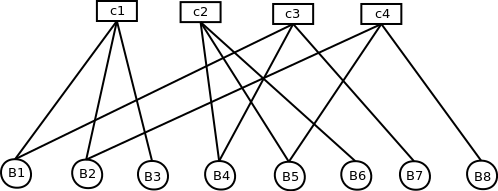
\includegraphics[height=4.5cm,width=10cm]{minSum1}
\caption[Tanner graph]{Tanner graph}
\end{figure}

\subsection{Sum Product Decoding\cite{9}}

The input bit probabilities are called the a priori probabilities.
The bit probabilities returned by the decoder are called the a posteriori probabilities.
For sum-product decoding these probabilities are expressed
as log-likelihood ratios (LLR).
\begin{align} L(x)=log\dfrac{p(x=0)}{p(x=1)}=log\dfrac{1-p(x=1)}{p(x=1)} \end{align}
 If p(x = 0) $>$ p(x = 1) then L(x) is positive.
%The greater the difference between p(x = 0) and p(x = 1), i.e. the more
%sure we are that p(x) = 0, the larger the positive value for L(x), and vic. versa.
%Log Likelihood Ratios are used to represent the metrics for a binary variable x
%by a single value rather than individual probability of being zero and one.
%The sign of L(x) provides the hard decision on x and the magnitude $|L(x)|$ represents
%the reliability of this decision.\\
%LLR based representation has benefit when probabilities
%Rneed to be multiplied LLR need only be added, reducing the implementation complexity.
T%he goal is to achieve maximum a posteriori probability of for each bit. 
The extra information about bit i received
from the parity-check j is called extrinsic information for bit i denoted by $E_{j,i}$. The probability ($P_{j,i}^{ext}$ ) that check j is satisfied when ith bit is one is equal to the probability of having odd number of 1s in the check j other than bit i.
\begin{align} P_{j,i}^{ext} = \dfrac{1}{2}-\dfrac{1}{2} \prod_{i'\in B_j, \ i'\neq i }(1-2P_{i'}^{int})  \end{align}
$P_{i'}^{int}$ is a priori probability of ith bit to be 1. Thus,
\[ E_{(j,i)} =  LLR (P_{j,i}^{ext}) = log \left(
\dfrac{1-P_{j,i}^{ext}}{P_{j,i}^{ext}} 
\right)
\]
\[ E_{(j,i)} = log
\left(
\dfrac{\dfrac{1}{2}+\dfrac{1}{2} \prod_{i'\in B_j \ i'\neq i }(1-2P_{i'}^{int}) }{\dfrac{1}{2}-\dfrac{1}{2} \prod_{i'\in B_j \ i'\neq i }(1-2P_{i'}^{int}) } 
\right)
 \]
Using relationship: $tanh \left(  \dfrac{1}{2}log \left( \dfrac{1-p}{p} \right) \right)=1-2p$;
\[ E_{(j,i)} = log
\left(
\dfrac{\dfrac{1}{2}+\dfrac{1}{2} \prod_{i'\in B_j \ i'\neq i }tanh(M_{j,i'}/2) }{\dfrac{1}{2}-\dfrac{1}{2} \prod_{i'\in B_j \ i'\neq i }tanh(M_{j,i'}/2) } 
\right)
 \]
where 
\[ M_{(j,i')} =  LLR (P_{j,i'}^{int}) = log \left(
\dfrac{1-P_{j,i'}^{int}}{P_{j,i'}^{int}} 
\right)
\]
Alternatively, using the relationship
\[ 2tan^{-1}(p)=log \left( \dfrac{1+p}{1-p} \right) \]
%%%%%%%%%%%%%%%%%%%%%%%%%%%%%%%%%%%%%%%%%%%%%
Thus extrinsic information from check j to bit i is:
\begin{align} E_{(j,i)} = 2tan^{-1} \left( \prod_{i'\in B_j ,\ i'\neq i }tanh(M_{j,i'}/2) \right) \end{align}
Total LLR passed to bit i is
\begin{align} L_i = LLR(P_i^{int}) = r_i + \sum_{j\in A_i} E_{j,i} \end{align}
where $r_i$ is input a priori for bit i.
But, message sent again from bit to check avoid the information which checks already have. Thus,
$M_{j,i}$ is not exactly the extrinsic information, it exclude the message generated by the same check node.\\
\begin{align}  M_{j,i} = \sum_{j'\in A_i j'\neq j} E_{j,i} + r_i \end{align}.\\
%\item %Each bit has access to the input a priori LLR, ri, and the LLRs from every
%connected check node. The total LLR of the i-th bit is the sum of these LLRs
     

After every iteration hard decision is made on the LLR post priori. If code satisfies $Hc^T=0$ then decoding stop else $M_{j,i}$ is found and next iteration is performed.
\subsection{Min Sum Decoding}
The min sum decode algorithm is simplification in the sum product algorithm. \\
For BPSK modulation transmitted $0's$ are represented as $-1s$ and transmitted $1s$ are represented as $1s$. \\
The probability that bit 1 is received 
\begin{align} f_y(y|f=-1) = \dfrac{1}{\sqrt{2\pi\sigma^{2}}} \exp{\dfrac{-(y+1)^2}{2\sigma^2}}
 \end{align}
 

The probability that bit 0 is received 
\begin{align} f_y(y|f=1) = \dfrac{1}{\sqrt{2\pi\sigma^{2}}} \exp{\dfrac{-(y-1)^2}{2\sigma^2}}
 \end{align}
 
Thus getting LLR as:
\begin{align}  LLR = \log\dfrac{f_y(y|f=-1)}{f_y(y|f=1)} = \dfrac{-2y}{\sigma^2}
 \end{align}
 
A priori information on the bit node side is expressed in term of LLR as: 
\begin{align}  aPriori[I] = -4 * C[I] * R * \dfrac{Eb}{No} 
 \end{align}
where C[I] = $i^{th}$ code block, R = code rate and 
$\dfrac{Eb}{No}$ = signal to noise power ratio\\
	
Messages are the information propagating from bit nodes to check nodes.
These are initialized to a priori of their respective bit node.	
\begin{align} message[I][J] = aPriori[I] 
 \end{align}
 
Extrinsic information of a bit node is calculated min sum of all the messages connected to 
	that particular check node. 
\begin{align} |E_{(j,i)}| =  Min_{i'\in B_j \ i'\neq i }|M_{j,i'}|   
 \end{align}

\begin{align} sign({E_{(j,i)}}) =  \prod_{i'\in B_j \ i'\neq i }sign(M_{j,i'})   
 \end{align}
 
A posteriori probabilities are the output bit probabilities.
These are used to modify the code block after every iteration.

\begin{align}  aPosteriori[I] = \sum_{j\in A_i} E_{j,i} + aPriori[I] 
 \end{align}
	
Then hard decision is taken on the a posteriori information, that represent the decoded code block.
If decoded code block satisfies $c*H^{T} = 0 $, then decoding stops. Else messages are updated and transmitted back to start the next iteration of decoding.
\begin{align}   message_{(j,i)} = aPosteriori[i] - E_{(j,i)}  
 \end{align}	



% Introduction

% Main chapter title
\chapter{C Level Implementation \& Verification} 

% Change X to a consecutive number; for referencing this chapter elsewhere, use \ref{ChapterX}
\label{Chapter4} 

% This is for the header on each page
\lhead{Chapter 4. \emph{Theory of LDPC}}  

We have implemented \textit{bit flipping algorithm}, \textit{sum product algorithm} and \textit{min sum algorithm} in C. \\
The decoding algorithms are so implemented that it can be used for any arbitrary rate and parity check matrix. The software takes parity check matrix file, code block file as input arguments and after decoding it writes decoded block in a file. The software can also compute time to decode and accuracy of decoding according to additional input argument given. \\

After developing the software for basic LDPC decoding algorithms in C we decided to convert min sum decode algorithm from C level description to hardware. This is done by Ahir tool chain, developed at IIT-Bomabay under the supervision of Prof. Madhav P. Desai. Firstly, we concentrated on testing algorithmic accuracy of min sum decode algorithm. The reason to verify the algorithm so regressively in C level is that it gives us confidence to proceed for the hardware design.  

\section{ Min Sum Decode Algorithm}
The key specification of the algorithm and notations on the tables are as follows :
\begin{itemize}
\item Min sum algorithm is implemented for Gaussian channel. 
\item Quasi-cyclic matrix of block size(n=) 4K, 8K and 12K  are formed using Sridhara-Fuja-Tanner algorithm.
\item Five different code rates(R=) 0.75, 0.80, 0.85, 0.90 and 0.95 are taken.
\item Raw input bit error rate(BER(IN)) is between $10^{-2}$ to $10^{-3}$, converted in form of Eb/No(db) to express input SNR in db. 
\item BER(OUT) : Output block error rate.
\item CDB : Number of correctly decoded blocks.  
\item Itr : Average number of iterations per block.
\end{itemize}



\subsection{Results on Quasi Cyclic Matrix}
\subsubsection{Block Error Rate }

We have sent code blocks continuously and noted when the first code block gets incorrectly decoded. Maximum number of sent blocks is 1 million. If all 1 million blocks gets correctly decoded then $'-'$ is shown in table.

\begin{table}[H]
\centering
\caption[Table for block error estimates of Min Sum decode using quasi cyclic matrix]{ Table for block error estimates  }
\begin{tabular}{|l|l|r|r|r|r|r|}
\hline
n$\simeq$   & BER(In)$\simeq$    & R=0.75  & R=0.80  & R=0.85  & R=0.9 & R=0.95 \\ \hline
4K  & $1.0\times10^{-2}$  & -    & - &2.677$\times10^{3}$           &1.7819$\times10^{4}$       &1       \\ 
    & $0.5\times10^{-3}$  &-     & - &2.4944$\times10^{4}$          &1.65511$x10^{5}$		&1.79$\times10^{2}$   \\ 
    & $1.0\times10^{-3}$  & -   & -  &5.47550$\times10^{5}$         &4.89654$\times10^{5}$     &3.328$\times10^{3}$ \\ \hline
8K  & $1.0\times10^{-2}$   & -   & - &2.3817$\times10^{4}$          &1.16847$\times10^{5}$        &1   \\ 
    & $0.5\times10^{-3}$   & -     & -&6.9491$\times10^{4}$          &1.72263$\times10^{5}$       &1.001$\times10^{3}$  \\ 
    & $1.0\times10^{-3}$   & -   & -  &9.16505 $\times10^{5}$        &6.28939$\times10^{5}$       &9.338$\times10^{3}$  \\ \hline
12K & $1.0\times10^{-2}$   & -   & -  &9.705$\times10^{3}$          &5.37754$\times10^{5}$       	&1       \\
    & $0.5\times10^{-3}$   & -     & -&5.6400$\times10^{4}$          &-     			 		&1.318$\times10^{3}$  \\ 
    & $1.0\times10^{-3}$   & - & - &- 			             &-    					 &1.6920$\times10^{4}$   \\ \hline 
\end{tabular}
\label{tab:nameForThisTable}
\end{table}

\subsubsection{ Error threshold  and number of iterations required  }
We have tabulated results for the test case when we send 100 code blocks and noted BER and number of iterations to decode.
The testing focus to get error threshold of the algorithm. Error threshold is the maximum input bit error rate that can be corrected by the decoder. We performed testing by varying input BER between $10^{-2}$ to $10^{-3}$. To get error threshold we check for the input BER at which no block gets correctly decoded when sending 100 code blocks are sent.  
\begin{table}[H]
\centering
\caption[Table for error threshold estimate at code rate = 0.75, Min Sum decode using quasi cyclic matrix]{Table for error threshold estimate at  code rate = 0.75 }
\begin{tabular}{|l|l|l|l|l|l|l|}
\hline
n     & BER(In) 			& Eb/No(db) & BER(OUT) & CDB  & Itr \\ \hline
4112  & $3.3\times10^{-2}$       & 3.5   & 0   & 100 & 5         \\  \hline
	  & $1.0\times10^{-2}$       & 5.5   & 0   & 100 & 2         \\ 
      &	$4.8\times10^{-3}$		& 6.5   & 0   & 100 & 1         \\
      &	$1.8\times10^{-3}$		& 7.5   & 0   & 100 & 1         \\ \hline
8180  &	$2.9\times10^{-2}$    	& 3.8   & 0   & 100 & 5         \\  \hline
      &	$1.0\times10^{-2}$    	& 5.5   & 0   & 100 & 2         \\ 
      &	$4.8\times10^{-3}$		& 6.5   & 0   & 100 & 1         \\
      &	$1.8\times10^{-3}$		& 7.5   & 0   & 100 & 1         \\ \hline
12304 &	$3.4\times10^{-2}$		& 3.4   & 0   & 100 & 6         \\ \hline
	  &	$1.0\times10^{-2}$		& 5.5   & 0   & 100 & 2         \\  
      &	$4.8\times10^{-3}$		& 6.5   & 0   & 100 & 1         \\ 
      &	$1.8\times10^{-3}$		& 7.5   & 0   & 100 & 1         \\ \hline
\end{tabular}
\label{tab:nameForThisTable}
\end{table}


\begin{table}[H]
\centering
\caption[Table for error threshold estimate at code rate = 0.95, Min Sum decode using quasi cyclic matrix]{Table for error threshold estimate at code rate = 0.95}
\begin{tabular}{|l|l|l|l|l|l|}
\hline
n     & BER(IN)& Eb/No(db) & BER    & CDB & Itr(/25) \\ \hline
4260  & $1.1\times10^{-2}$ & 4.5   & $6.8\times10^{-3}$      & 23 &  -       \\ 
      & $4.7\times10^{-3}$ & 5.5   & 0           & 100 & 3         \\  
      & $1.6\times10^{-3}$ & 6.5   & 0           & 100 & 2         \\ \hline
8220  & $1.1\times10^{-2}$ & 4.5   & $7.5\times10^{-3}$      & 8 & -         \\ 
      & $4.7\times10^{-3}$ & 5.5   & $2.8\times10^{-7}$      & 99 & -         \\ 
      & $1.6\times10^{-3}$ & 6.5   & 0      & 100 & 2         \\ \hline
12660 & $1.1\times10^{-2}$ & 4.5   & $7.2\times10^{-3}$      & 4 & -        \\ 
      & $4.7\times10^{-3}$ & 5.5   & 0      & 100 & 4         \\ 
      & $1.6\times10^{-3}$ & 6.5   & 0      & 100 & 2         \\ \hline      
\end{tabular}
\label{tab:nameForThisTable}
\end{table}

\begin{table}[H]
\centering
\caption[Table for error threshold estimate at code rate = 0.80, Min Sum decode using quasi cyclic matrix]{Table for error threshold estimate at code rate = 0.80}
\begin{tabular}{|l|l|l|l|l|l|}
\hline
n     & BER(In)  	& Eb/No(db) & BER & CDB & Itr(/25) \\ \hline
4075  &	$2.2\times10^{-2}$ & 4.1   & 0   & 100 & 4         \\  \hline
	  &	$0.8\times10^{-2}$ & 5.5   & 0   & 100 & 2         \\
      &	$3.8\times10^{-3}$ & 6.5   & 0   & 100 & 1         \\ 
      &	$1.5\times10^{-3}$ & 7.5   & 0   & 100 & 1         \\ \hline
8275  &	$2.4\times10^{-2}$ & 3.9   & 0   & 100 & 5         \\  \hline
	  &	$0.8\times10^{-2}$ & 5.5   & 0   & 100 & 2         \\ 
      &	$3.8\times10^{-3}$ & 6.5   & 0   & 100 & 1         \\ 
      &	$1.5\times10^{-3}$ & 7.5   & 0   & 100 & 1         \\ \hline
12275 &	$2.5\times10^{-2}$ & 3.8   & 0   & 100 & 6         \\ \hline
      &	$0.8\times10^{-2}$ & 5.5   & 0   & 100 & 2         \\  
      &	$3.8\times10^{-3}$ & 6.5   & 0   & 100 & 1         \\
      &	$1.5\times10^{-3}$ & 7.5   & 0   & 100 & 1         \\ \hline
\end{tabular}
\label{tab:nameForThisTable}
\end{table}



\begin{table}[H]
\centering
\caption[Table for error threshold estimate at code rate = 0.85, Min Sum decode using quasi cyclic matrix]{Table for error threshold estimate at code rate = 0.85}
\begin{tabular}{|l|l|l|l|l|l|}
\hline
n     & BER(IN) & Eb/No(db) & BER & CDB & Itr(/25) \\ \hline
4220  & $1.9\times10^{-2}$ & 4     & 0   & 100 & 6         \\ \hline
	  & $1.0\times10^{-2}$ & 5     & 0   & 100 & 3         \\
      & $4.5\times10^{-3}$ & 6     & 0   & 100 & 2         \\ 
      & $1.7\times10^{-3}$ & 7     & 0   & 100 & 1         \\ \hline
8180  & $1.9\times10^{-2}$ & 4     & 0   & 100 & 6         \\  \hline
      & $1.0\times10^{-2}$ & 5     & 0   & 100 & 3         \\ 
      & $4.5\times10^{-3}$ & 6     & 0   & 100 & 2         \\ 
      & $1.7\times10^{-3}$ & 7     & 0   & 100 & 1         \\ \hline
12260 & $1.9\times10^{-2}$ & 4     & 0   & 100 & 6         \\  \hline
      & $1.0\times10^{-2}$ & 5     & 0   & 100 & 3         \\ 
      & $4.5\times10^{-3}$ & 6     & 0   & 100 & 2         \\ 
      & $1.7\times10^{-3}$ & 7     & 0   & 100 & 1         \\ \hline
\end{tabular}
\label{tab:nameForThisTable}
\end{table}


\begin{table}[H]
\centering
\caption[Table for error threshold estimate at code rate = 0.90, Min Sum decode using quasi cyclic matrix]{Table for error threshold estimate at code rate = 0.90}
\begin{tabular}{|l|l|l|l|l|l|}
\hline
n     & BER(IN) & Eb/No(db) & BER & CDB & Itr(/25) \\ \hline
4120  & $1.1\times10^{-2}$ & 4.7     & 0   & 100 & 4         \\  \hline
      & $0.9\times10^{-2}$ & 5     & 0   & 100 & 3         \\ 
      & $3.6\times10^{-3}$ & 6     & 0   & 100 & 2         \\ 
      & $1.3\times10^{-3}$ & 7     & 0   & 100 & 1         \\ \hline
8440  & $1.2\times10^{-2}$ & 4.5     & 0   & 100 & 5         \\  \hline
      & $0.9\times10^{-2}$ & 5     & 0   & 100 & 3         \\ 
      & $3.6\times10^{-3}$ & 6     & 0   & 100 & 2         \\ 
      & $1.3\times10^{-3}$ & 7     & 0   & 100 & 1         \\ \hline
12280 & $1.2\times10^{-2}$ & 4.5     & 0   & 100 & 5         \\  \hline
      & $0.9\times10^{-2}$ & 5     & 0   & 100 & 3         \\ 
      & $3.6\times10^{-3}$ & 6     & 0   & 100 & 2         \\ 
      & $1.3\times10^{-3}$ & 7     & 0   & 100 & 1         \\ \hline
\end{tabular}
\label{tab:nameForThisTable}
\end{table}

\begin{table}[H]
\centering
\caption[Table for error threshold estimate at code rate = 0.95, Min Sum decode using quasi cyclic matrix]{Table for error threshold estimate at code rate = 0.95}
\begin{tabular}{|l|l|l|l|l|l|}
\hline
n     & BER(IN)& Eb/No(db) & BER    & CDB & Itr(/25) \\ \hline
4260  & $1.1\times10^{-2}$ & 4.5   & $6.8\times10^{-3}$      & 23 &  -       \\ 
      & $4.7\times10^{-3}$ & 5.5   & 0           & 100 & 3         \\  
      & $1.6\times10^{-3}$ & 6.5   & 0           & 100 & 2         \\ \hline
8220  & $1.1\times10^{-2}$ & 4.5   & $7.5\times10^{-3}$      & 8 & -         \\ 
      & $4.7\times10^{-3}$ & 5.5   & $2.8\times10^{-7}$      & 99 & -         \\ 
      & $1.6\times10^{-3}$ & 6.5   & 0      & 100 & 2         \\ \hline
12660 & $1.1\times10^{-2}$ & 4.5   & $7.2\times10^{-3}$      & 4 & -        \\ 
      & $4.7\times10^{-3}$ & 5.5   & 0      & 100 & 4         \\ 
      & $1.6\times10^{-3}$ & 6.5   & 0      & 100 & 2         \\ \hline      
\end{tabular}
\label{tab:nameForThisTable}
\end{table}

\subsection{Results on Random Matrices }
\subsubsection{Block Error Rate }

We have sent code blocks continuously and noted when the first code block gets incorrectly decoded. Maximum number of sent blocks is 1 million. If all 1 million blocks get correctly decoded then $'-'$ is shown in table.
\begin{table}[H]
\centering
\caption[Table for block error estimates of Min Sum decode using random matrix]{ Table for block error estimates  }
\begin{tabular}{|l|l|r|r|r|r|r|}
\hline
n$\simeq$   & BER(In)$\simeq$    & R=0.75  & R=0.8   & R=0.85  & R=0.9 & R=0.95 \\ \hline
4K  & $1.0\times10^{-2}$  &  1.2799$\times10^{4}$   & 2.0754$\times10^{4}$  & 3.39$\times10^{2}$ & 1.259$\times10^{3}$ & NA      
\\ 
    & $0.5\times10^{-3}$  &  5.53727$\times10^{5}$  &  1.72781$\times10^{5}$& 6.6700$\times10^{4}$ & 1.65511$\times10^{5}$ & NA   
\\ 
    & $1.0\times10^{-3}$  & -			      & 6.24436$\times10^{5}$& 3.45503$\times10^{5}$& 1.19008$\times10^{5}$  & NA  
\\ \hline
8K  & $1.0\times10^{-2}$  & 1.92476$\times10^{5}$   & 8.3898$\times10^{4}$  & 5.193$\times10^{3}$ & 5.947$\times10^{3}$         & NA      \\ 
    & $0.5\times10^{-3}$ & 3.21027$\times10^{5}$    & 4.6092$\times10^{4}$& 3.7952$\times10^{4}$ & 1.1389$\times10^{4}$ & NA  
\\ 
    & $1.0\times10^{-3}$ & -				     & -  				 & -         	  & -    & NA             
\\ \hline
12K & $1.0\times10^{-2}$ & 2.20022$\times10^{5}$   & 1.57371$\times10^{5}$  & 1.2894$\times10^{4}$ & 1.2626$\times10^{4}$     & 1.1      \\ 
    & $0.5\times10^{-3}$ & 2.17452$\times10^{5}$   & 9.0158$\times10^{4}$& 1.56487$\times10^{5}$& 5.4866$\times10^{4}$ & 1.034$\times10^{4}$    \\ 
    & $1.0\times10^{-3}$ & -				     & -   & -			  			 & -     & 1.4759$\times10^{4}$   \\ \hline
\end{tabular}
\label{tab:nameForThisTable}
\end{table}
For rate = 0.95 \& n = 4K,8k - we were not able to generate cycle-4 free parity check matrix.




 


% Introduction

% Main chapter title
\chapter{Partitioning of Tanner Graph} 

% Change X to a consecutive number; for referencing this chapter elsewhere, use \ref{ChapterX}
\label{Chapter6} 

% This is for the header on each page
\lhead{Chapter 5. \emph{Partitioning of Tanner Graph}}  

\section{Introduction}
The literature survey about hardware implementation of the LDPC decoder concludes three different implementation strategies.The serial decoder is the simplest decoder. Hardware cost and complexity is very less. It consists of single check node, single bit node and memory. The bits are first passed one by one from bit side to check side and generated checks are stored in memory, then checks are passed from check side to bit side one at a time to update the bit nodes. The main drawback is this implementation is too slow \cite{4}. The second approach is implementing a fully parallel algorithm. This is a direct implemention of the Tanner graph in hardware [5]. This increases the decoding speed, but hardware cost and implementation complexity becomes too high. Another approach is midway between serial and parallel, called partial parallel implementation. This implementation is more flexible as trade off between speed and cost can be done. In partial parallel implementation bit nodes and check nodes are divided into several partitions. All these partitions works in parallel, but within one partition the information is transferred serially. Larger the number of partitions, faster the decoder as it acts more like parallel decoder. Fewer the partitions, simpler the decoder as it acts more like serial implementation of the decoder. Thus, we can trade off between speed and cost. Further, a reconfigurable interconnection network has to be designed to change the connection from bit to check side for different iterations in partial parallel decoder. The multistage interconnection network provides cost efficient parallel processing. Non-blocking and rearrangable networks are preferred. In blocking network connection is not always possible, whereas non-blocking network always provides a path between input to output. A rearrangable network can always provide a path, but path has to be rearranged. Lee and Ryu have used Benes network in their partial parallel LDPC decoder \cite{5}. Benes network is a rearrangable network.

\section{Partitioning}
To use the partial parallel approach we propose to iteratively decompose the Tanner graph into sets of bits and sets of checks. In one iteration one set of bits is transferred towards one set of checks. It will be preferred that maximum number of the computational bits required for a particular check set are in same bit set so that computation can be completed for as many check nodes as possible. If a check set requires bits from many bit sets, then the number of iterations required to complete the computation of that set will be equal to the number of bit sets required to perform all the computation. Thus, if many check sets require bits from a large number of bit sets, then number of iterations increases and decoding time will become worse. Thus, an efficient partitioning of bit and check side of the Tanner graph is required. \\
The objective is to partition the bipartite graph corresponding to parity check matrix into two subsets in both bit side and check side such that most of the edges of a set of bit side relates to a particular set of check side. We call these edges as \lq Through edges\rq. The remaining edges of the same set on the bit side that goes to different set in check side are called \lq Transverse edges\rq. The average ratio of total number
of through edges to total number of edges is the performance index for parallelization. \\
Suppose we have bipartite graph G, bits are
B = \{ $b_{1}$ , $ b_{2}$ ,$b_{3}$ ,...,$b_{n}$ \} and checks are C=\{ $c_{1}$,$c_{2}$ ,$c_{3}$,...,$c_{m}$ \}
and the edge between bit node $b_{i}$ and check node $c_{j}$ is represented as $e{i,j}$. Now we have to partition G into four subsets $B_{1}$ ,$B_{2}$ ,$C_{1}$ and $C_{2}$ such that
\begin{itemize}
\item   Size of set$ B_{1}$ and set $B_{2}$ should be nearly equal as well
as size of$ C_{1}$ $and C_{2}$ should be nearly equal.
\item  There should be a very small number of edges between
$B_{1}$-$C_{2}$and $B_{2}$-$C_t{1}$so that the number of cross edges are minimised. 
\end{itemize}


 \begin{figure}[h]
 \begin{center}
    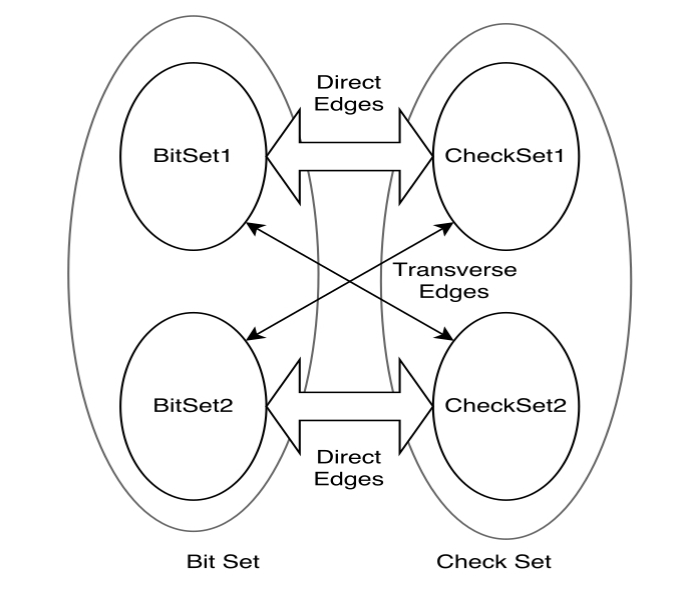
\includegraphics[height=8cm,width=8cm]{partition1.jpg}
    \caption{Partitioning a bipartite graph} 
 \end{center}
\end{figure}


\section{Procedure}
To approach this we initially find a weighted check matrix from the parity check matrix. The weighted check matrix is an incidence matrix for the check node graph. A check node graph is a weighted graph. The weight between $checknode_{i}$ and $checknode_{j}$ is the number of common bit nodes performing check on both $checknode_{i}$ and $checknode_{j}$ . After forming the
weighted check graph we partitioned it into two equal parts using METIS \cite{6}. After partitioning the check set into two equal sets with minimum weight cut, we need to partition the bit set. To partition the bit set we take into account the number of checks associated with a bit. If number of checks associated with a bit are more in first check set then it goes to first check set else it goes to second check set. As all matrices are sparse, the number of bits divided in two sets comes out nearly equal. To make them exactly equal we force some bits to go to other set after partitioning. Then the average ratio of parallelized edges to total edges and transverse edges to total edges is calculated as a performance index of parallelization of the
decoder. Figure \ref{partition2} shows the block diagram for the process of partitioning the bipartite graph corresponding to a low density parity check matrix.


 \begin{figure}[h]
 \begin{center}
    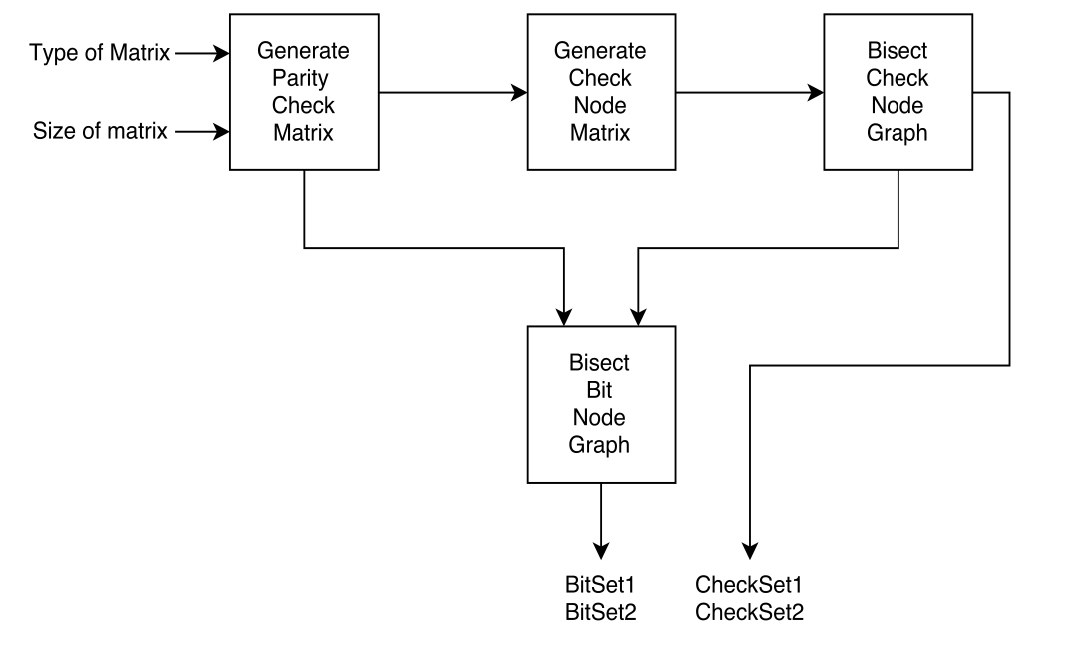
\includegraphics[height=8cm,width=14cm]{partition2.jpg}
    \caption{Block Diagram of process flow} 
    \label{partition2}
 \end{center}
\end{figure}  

\begin{itemize}
\item \textbf{Generation of Parity Check Matrix}
\item \textbf{Generation of Check Node Incident Matrix} \\
The weight between two check nodes is the number of common bit nodes performing exor operation on both check nodes.
Taking this into account, we followed following algorithm to
convert a parity check matrix to a check node incidence matrix.

\item \textbf{Bisection of Check Node Graph}

Partitioning of check node graph is done using METIS \cite{6}.
"METIS is a set of serial programs for partitioning graphs,
partitioning finite element meshes, and producing fill reducing
ordering for sparse matrices. The algorithms implemented in
METIS are based on the multilevel recursive-bisection, multilevel k-way, and multi-constraint partitioning schemes"\cite{6}.
First, the incidence matrix is converted into a corresponding
graph format that can be given as input to METIS. At output
we get two partitions of equal size with the minimum weight
cut.

\item \textbf{Bisection of Bit Node Graph}

After bisection of the check set we get two sets $C_{1}$ and $C_{2}$ .
Now, we have to divide a partition of bit set into $B_{1}$ and $B_{2}$ . A
bit node corresponds to set $ B_{1}$ if the number of edges between
that bit node and set $C_{1}$ are more than the number of edges
between bit node and set $ C_{2}$ . As the check set is bisected by
keeping in mind that the more the number of checks relating
to a bit are in same set and the matrix is sparse thus we get
nearly equal bits in set $B_{1}$ and set $B_{2}$. As this bisection has
to be further iterated for partitioning, we force the bisection
to be equal. Forcing the bisection to be equal increases the
transverse edges.


\end{itemize}

\section{Results of partitioning applied to matrices}
Simulation for partitioning are performed in MATLAB environment. Figure \ref{gallager_part} shows the performance index for Gallager matrix when we vary the order of the parity check matrix from 1,000 to 10,000. The performance index comes 0.78 for Gallager matrix. Similarly, by varying the order of the parity check matrix from 1,000 to 10,000 we get performance index of MacKay Neal matrix as 0.88, depicted in Figure \ref{makey_part}. Quasi Cyclic matrix can be formed only for a special set of numbers. In simulation, the order of matrix taken are 155, 305, 905 and 11555,
and performance index is above 0.88 in all cases, as depicted in Figure \ref{qc_part}.

 \begin{figure}[h]
 \begin{center}
    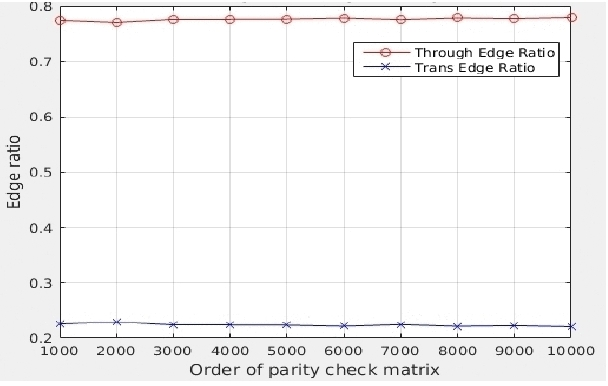
\includegraphics[height=8cm,width=12cm]{gallager_part.jpg}
    \caption{Performance of Gallager matrix}
    \label{gallager_part} 
 \end{center}
\end{figure}   
 
  \begin{figure}[h]
 \begin{center}
    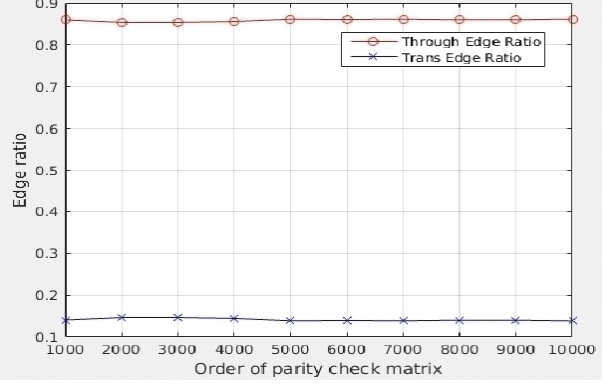
\includegraphics[height=8cm,width=12cm]{makey_part.jpg}
    \caption{Performance of MacKay Neal matrix} 
    \label{makey_part}
 \end{center}
\end{figure}


 \begin{figure}[h]
 \begin{center}
    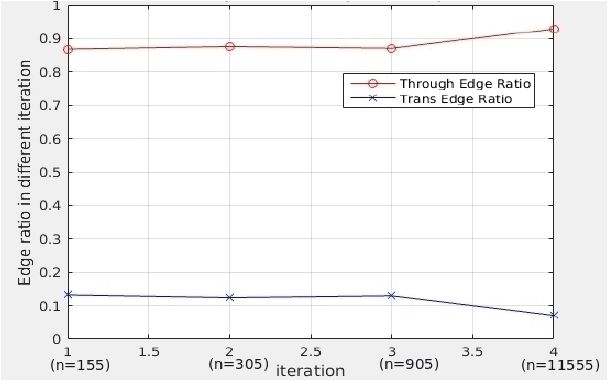
\includegraphics[height=8cm,width=12cm]{qc_part.jpg}
    \caption{Performance of quasi-cyclic matrix} 
    \label{qc_part}
 \end{center}
\end{figure}

% Introduction

% Main chapter title
\chapter{Modification in Min Sum Algorithm using partitioning}

% Change X to a consecutive number; for referencing this chapter elsewhere, use \ref{ChapterX}
\label{Chapter7} 

% This is for the header on each page
\lhead{Chapter 6. \emph{Proposed modification in Min Sum Algorithm using partitioning}}  

The idea is to modify the min sum algorithm such that we can deploy it in a partitioned matrix iteratively to decode a code block.
To state the modification we first explain min sum algorithm by a example and then we show the modification in it:

\section{Example explaining min sum decode }
The parity check matrix chosen to decode the code block is as following.
\[
\left[ \begin{array} {c|cccccccc} 
  &    c1 &   c2 &   c3 &  c4  &  c5  &  c6  &  c7  &  c8 \\ \hline
r1 &    1  &   1  &   1  &   0  &   0  &   0  &   0  &   0 \\
r2 &    0  &   0  &   0  &   1  &   1  &   1  &   0  &   0 \\ 
r3 &    1  &   0  &   0  &   1  &   0  &   0  &   1  &   0 \\
r4 &    0  &   1  &   0  &   0  &   1  &   0  &   0  &   1 \end{array} \right] 
\]			
The Tanner graph corresponding to above parity check  matrix is depicted in figure \ref{Tanner Graph}.
\\
\begin{figure}[h!]
\centering
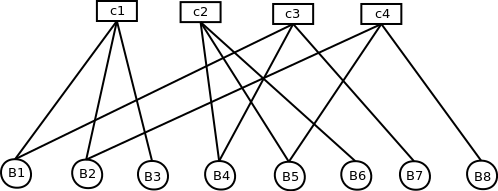
\includegraphics[height=5cm,width=12cm]{minSum1}
\caption[Tanner Graph]{Tanner Graph}
\label{Tanner Graph}
\end{figure}

The code block received at the receiver is represented by C. The SNR at the input of receiver is represented as $\dfrac{E_{b}}{No}$. The code is represented as R.
\\
\textbf{Step 1:} We calculate the a priori probabilities at the receiver end. A priori probability of a particular code bit is the log likelyhood ratio of the code bit.
\[  aPriori[I] = -4 * C[I] * R * \dfrac{Eb}{No} \]
Assuming we get the a priori probability = \{ -3.2 , 2.8 , -3.6 , 2.8 , 2 , -6 , - 9.6 , -4.8 \}
\begin{figure}[h!]
\centering
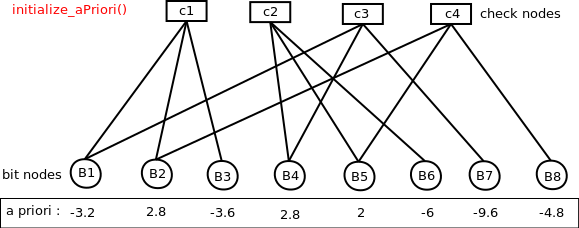
\includegraphics[height=6cm,width=12cm]{minSum2}
\caption[Initialization of a priori probabilities ]{Initializing a priori probabilities}
\label{minSum2}
\end{figure}
\\
\textbf{Step 2:}
We calculate messages transferred from bit nodes to check nodes through the edges of Tanner graph as depicted in figure \ref{minSum3}
 \[ message[I][J] = aPriori[I] \]
\begin{figure}[h!]
\centering
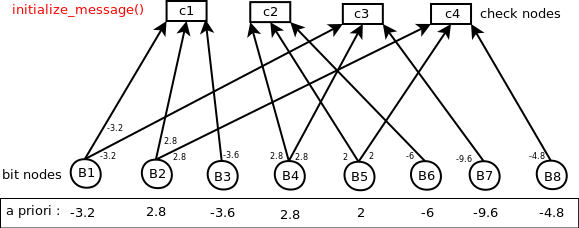
\includegraphics[height=6cm,width=12cm]{minSum3}
\caption[Initialization of messages]{Initializing messages}
\label{minSum3}
\end{figure}

\textbf{Step 3:}
We calculate extrinsic information at the check nodes and transfer the information back to the bit nodes through edges as depicted in figure \ref{minSum4}
 \[ |E_{(j,i)}| =  Min_{i'\in B_j \ i'\neq i }|M_{j,i'}|   \] 
 \[ sign({E_{(j,i)}}) =  \prod_{i'\in B_j \ i'\neq i }sign(M_{j,i'})   \]
\begin{figure}[h!]
\centering
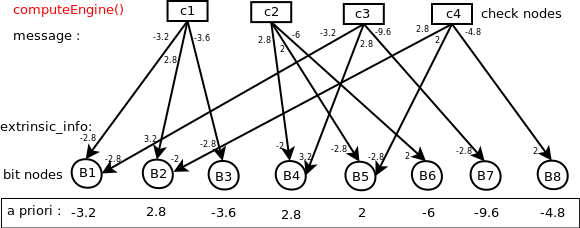
\includegraphics[height=6cm,width=12cm]{minSum4}
\caption[Computation of extrinsic information]{Computing extrinsic information}
\label{minSum4}
\end{figure}

\textbf{Step 4:}
After computation of extrinsic informations we calculate a posteriori probabilities at each bit nodes as depicted in figure \ref{minSum5}
\begin{figure}[h!]
\centering
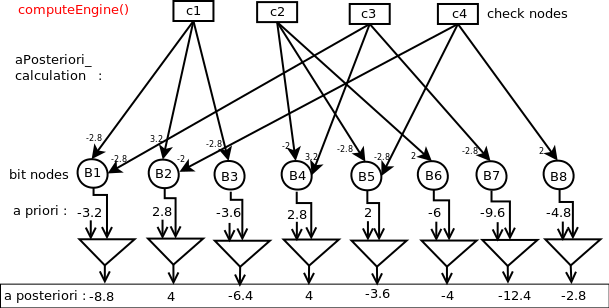
\includegraphics[height=8cm,width=12cm]{minSum5}
\caption[Calculation of a posteriori probabilities]{Calculating a posteriori probabilities}
\label{minSum5}
\end{figure}

\textbf{Step 5:}
A posteriori probabilities are the estimate of the code bits. Thus we take hard decision on the a posteriori probabilities. And this new estimate of code block is compared to the present code block. If both are same  then decoding stops. 

\textbf{Step 6:}
Else, we modify the code bits and messages and start the next iteration to decode the code block. The messages are updated as shown is figure \ref{minSum7}
\begin{figure}[h!]
\centering
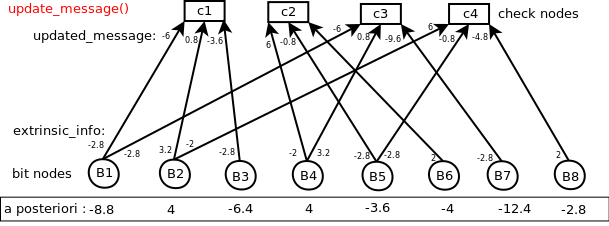
\includegraphics[height=6cm,width=12cm]{minSum7}
\caption[Updating the messages]{Updating the messages}
\label{minSum7}
\end{figure}

\section{ Example explaining modifications on min sum decode algorithm for a partitioned matrix }

As we have partitioned the matrix the parity check matrix looks as follows.
\[
H = \left[ \begin{array}{c|c}  
H11  & H12     \\ \hline
H21  & H22     \end{array} \right] 
\] 
\[
\left[ \begin{array} {c|cccccccc} 
  &    c1 &   c2 &   c3 &  c4  &  c5  &  c6  &  c7  &  c8 \\ \hline
r1 &    1  &   1  &   1  &   0  &   0  &   0  &   0  &   0 \\
r2 &    0  &   0  &   0  &   1  &   1  &   1  &   0  &   0 \\ 
r3 &    1  &   0  &   0  &   1  &   0  &   0  &   1  &   0 \\
r4 &    0  &   1  &   0  &   0  &   1  &   0  &   0  &   1 \end{array} \right] 
     \Rightarrow
\left[ \begin{array} {c|cccc|cccc} 
  &    c4 &   c6 &   c7 &  c1  &  c2  &  c3  &  c8  &  c5 \\ \hline  
r2 &     1  &   1  &   0  &   0  &   0  &   0  &   0  &   1 \\
r3 &     1  &   0  &   1  &   1  &   0  &   0  &   0  &   0 \\ \hline
r1 &     0  &   0  &   0  &   1  &   1  &   1  &   0  &   0 \\
r4 &     0  &   0  &   0  &   0  &   1  &   0  &   1  &   1 \end{array} \right] 
\]

\textbf{Step 1:} 
Assuming we get the a priori probabilities = \{ 5.59 , -11.99 , -19.19 , -6.39 , 5.59 , -7.1 , - 9.59 , 3.99 \}. The a priori initialization is shown in figure \ref{minSumModified1}
\begin{figure}[h!]
\centering
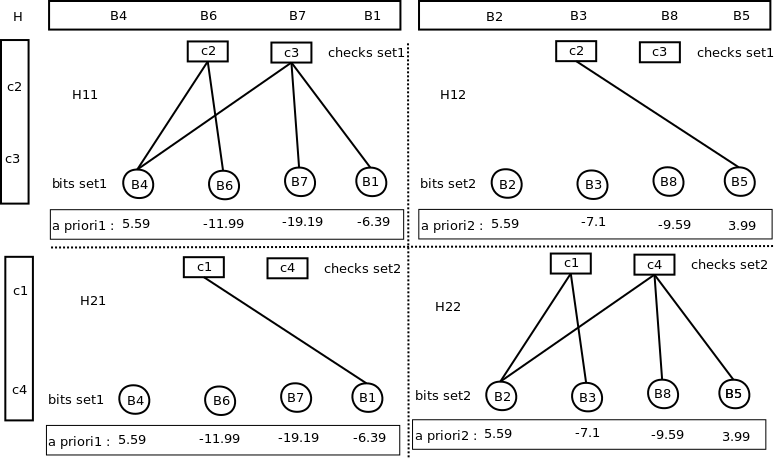
\includegraphics[height=8cm,width=12cm]{minSumModified1}
\caption[Initialization of a priori probabilities on  partitioned Tanner graphs]{Initializing a priori probabilities on partitioned Tanner graphs}
\label{minSumModified1}
\end{figure}
\\
\textbf{Step 2:}
The message initialization is done similarly and is  depicted in figure \ref{minSumModified2}
\begin{figure}[h!]
\centering
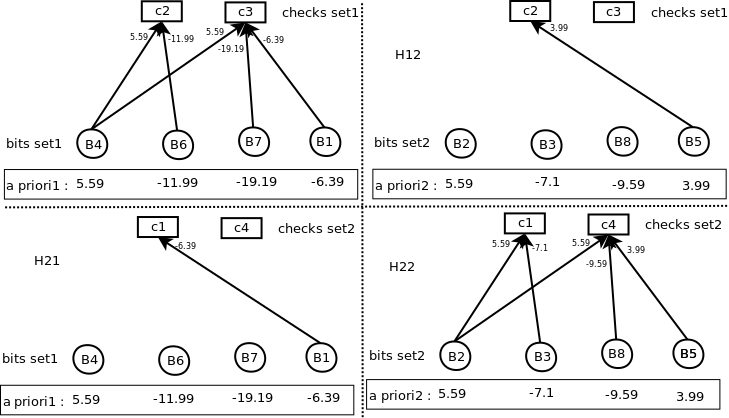
\includegraphics[height=8cm,width=12cm]{minSumModified2}
\caption[Initialization of messages on  partitioned Tanner graphs]{Initializing messages on  partitioned Tanner graphs}
\label{minSumModified2}
\end{figure}
\\
\textbf{Step 3:}
The computation of extrinsic information is broken into two parts. First we calculate partial extrinsic information at each matrix separately. At the same time we compute the transverse information required to calculate complete information from one check matrix to other check matrix, as depicted in figure  \ref{minSumModified3}

\begin{figure}[h!]
\centering
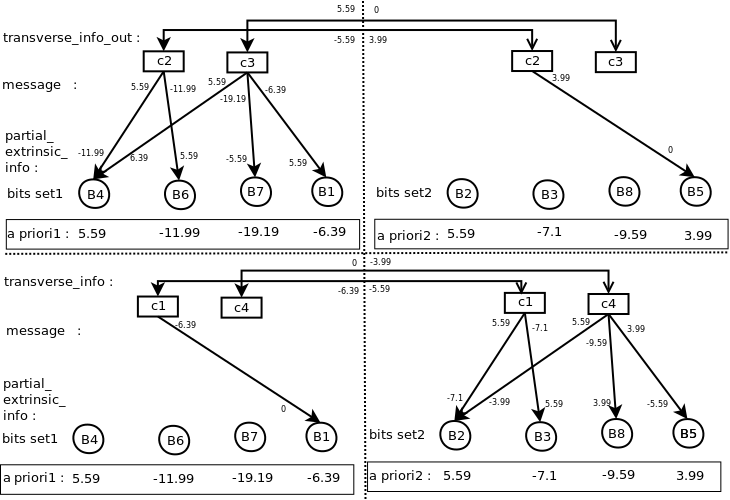
\includegraphics[height=8cm,width=12cm]{minSumModified3}
\caption[Computation of partial extrinsic information \& Transverse information ]{Computing partial extrinsic information \& Transverse information}
\label{minSumModified3}
\end{figure}

\textbf{Step 4:}
Then extrinsic information computation is completed by the transverse information as depicted in figure \ref{minSumModified4}
\begin{figure}[h!]
\centering
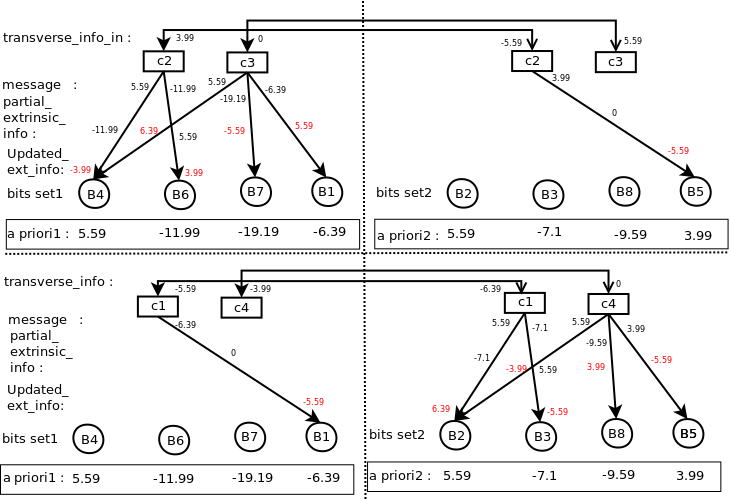
\includegraphics[height=8cm,width=12cm]{minSumModified4}
\caption[Computation of extrinsic information using Transverse information]{Computing extrinsic information using Transverse information}
\label{minSumModified4}
\end{figure}

\textbf{Step 5:}
A posteriori probabilities are  calculated similarly and the following steps of the algorithms remain the same. 

\section{ Modified Min Sum Algorithm }

By partitioning the matrix we can start computation in each matrix in parallel. This gives the hopes to parallelize the system and reduce the overall computation time. But the problem is that the computation on the partitioned matrix is not totally independent of the other matrices. Thus, the goal is to reduce the overall dependency of the computation in one partition of the matrix with the other partition of the matrix. The results after partitioning are shown in chapter 6 .The results are promising to get the desired behaviour. \\

The modification is essentially breaking the computation of extrinsic informations into multiple parts. The example explained that for a two way partition we have to break the computation in two stages. Similarly for a n-way partition we can break the computation in n stages. The trade off lies between number of stages and the number of computation engines. \\

For a two way partitioned matrix, the extrinsic information calculation is broken into two stages as following.
\\
\textbf{Stage 1:}
Partial extrinsic informations are calculated as for every matrix as following :
\begin{align}
|Ep_{(j,i)}| =  Min_{i'\in B_j \ i'\neq i }|M_{j,i'}|                                                                 
\end{align} 

\begin{align}
 sign({Ep_{(j,i)}}) =  \prod_{i'\in B_j \ i'\neq i }sign(M_{j,i'})  
\end{align} 
And the transverse corrections are calculated as following :

Transverse corrections is the information transferred between computation engines that shares common check nodes. Thus, these are computed for each check node. 
\begin{align} |T_{(j)}| =  Min_{i'\in B_j }|M_{(j,i')}|  
\end{align}  
\begin{align} sign({T_{(j)}}) =  \prod_{i'\in B_j}sign(M_{(j,i')})  
\end{align} 
 
\textbf{Stage 2:}
By using transverse information we calculate the net extrinsic information. 
\begin{align} |E_{(j,i)}| =  Min {|Ep_{(j,i')}| ,|T_{(j)}| }  
\end{align} 
\begin{align} sign({E_{(j,i)}}) =  \prod{sign(Ep_{(j,i')},sign(T_{(j)})  }
\end{align} 

Just keep in mind extrinsic information of a particular check node in a particular matrix depends upon partial extrinsic information of the same check node calculated in stage 1 by the same matrix, but transverse information of the matrix that shares the common check node. \\
As explained in the above example transverse information is transferred from $H_{(1,1)}$ to $H_{(1,2)}$ and vice versa. Similarly from  $H_{(2,1)}$ to $H_{(2,2)}$ and vice versa to compute the overall extrinsic information. \\

Thus if we generalise the concept for n-way partitioned matrix we just need to calculate the partial extrinsic information in stage 1. And then in subsequent stages we have to take in account the transverse information computed by same check node in all other n-1 partitioned matrices, that shares common check node. Thus we need a total number of n stages for a n-way partitioned matrix.


% Introduction

% Main chapter title
\chapter{ Hardware Implementation of the algorithms }

% Change X to a consecutive number; for referencing this chapter elsewhere, use \ref{ChapterX}
\label{Chapter8} 

% This is for the header on each page
\lhead{Chapter 7. \emph{Hardware Implementation of the algorithms \& Results}}

The algorithms are written in Aa language. The Aa description is then converted into vhdl using AHIR-tool-chain.\cite{8}


\section{Results}
The designs are characterised by two parameters. First parameter is number of clock cycles required to complete the decoding process or the time required to complete one iteration of decoding. Second parameter is the hardware required to implement the design. By this way we can compare the designs and opt a better trade off between cost verses performance.


 \begin{figure}[h]
 \begin{center}
    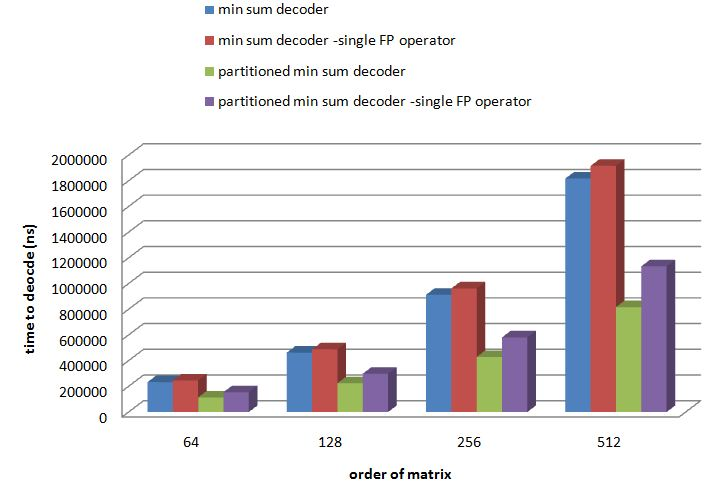
\includegraphics[height=8cm,width=12cm]{result_time.jpg}
    \caption{Comparison of time taken to decode} 
    \label{result_time}
 \end{center}
\end{figure}


Figure \ref{result_time} shows the time taken to decode for all the implemented designs for various order of matrices. The matrices used are randomly generated parity check matrices. The code rate is taken as half. Figure \ref{result_time} concludes that partitioned min sum decoder can decode approximately at half the time as compared to min sum decoder. \\
A floating point operation is very costly. Thus to reduce the cost of hardware we can also use single floating point operator. Its a trade off between cost verses performance. Figure \ref{result_time} shows that, if for both decoders we use shared floating point operator then the time to decode increases.  
 \begin{figure}[h]
 \begin{center}
    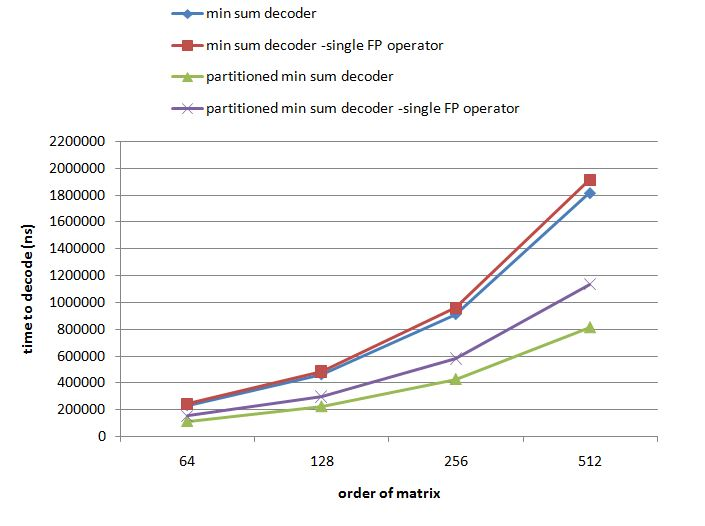
\includegraphics[height=8cm,width=12cm]{result_time1.jpg}
    \caption{Timing trends as the function of order of matrix} 
    \label{result_time1}
 \end{center}
\end{figure}

Figure \ref{result_time1} shows the variation of time to decode as the function of order of matrix. This concludes that the time to decode increases linearly with the order of matrix. \\


The hardware to implement the designs can be compared using Table \ref{result_hw}

\begin{table}[H]
\centering
\caption[Comparison of  hardware generated after implementing the designs]{ Comparison of  hardware generated after implementing the designs }
\begin{tabular}{|p{1.3cm}|p{3.5cm}|p{3.5cm}|p{3.5cm}|p{3.5cm}|}
\hline
	& min sum decoder & min sum decoder \newline
	(single FP unit) & partitioned min sum decoder & partitioned min sum decoder(single FP unit) \\ \hline
FF & 18,076		&19,034		&49,854		&55,988 \\ \hline
LUT & 19,502  &20,621 &  51,929 & 60,296 \\ \hline
Memory LUT & 6 & 3 & 23 & 2 \\ \hline 
I/O & 128 & 128 & 128 & 128 \\ \hline
BRAM & 56 & 56 & 80 & 80 \\ \hline
BUFG  & 1 & 1 & 1 & 1 \\ \hline
\end{tabular}
\label{result_hw}
\end{table}

 \begin{figure}[h]
 \begin{center}
    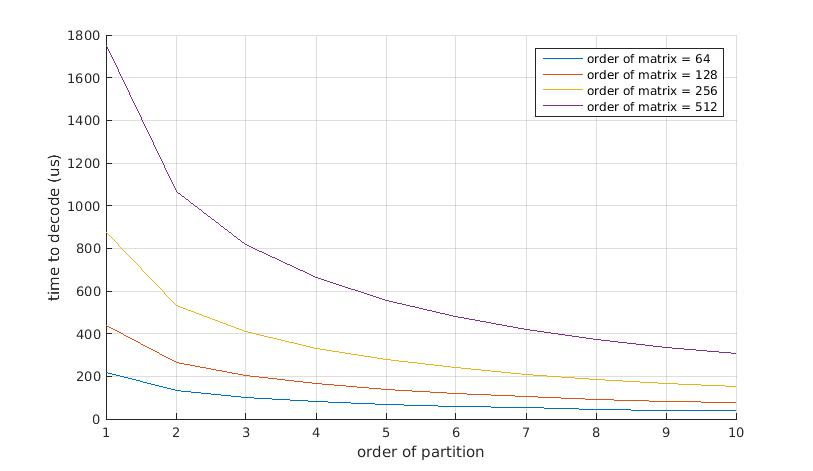
\includegraphics[height=8cm,width=12cm]{untitled.jpg}
    \caption{Timing trends as the function of order of partition} 
    \label{untitled}
 \end{center}
\end{figure}

Figure \ref{untitled} shows the time to decode the code block as a function of order of partitioning. The plot shows that for n-way partitioning of parity check matrix the time to decode reduce by a factor of n. The matrix used are random and have rate of half.



% Main chapter title
\chapter{Conclusion $\&$ Future Work}

% Change X to a consecutive number; for referencing this chapter elsewhere, use \ref{ChapterX}
\label{Chapter9} 

% This is for the header on each page
\lhead{Chapter 9. \emph{Conclusion $\&$ Future Work}}

Partitioning can help to improve the performance of the min sum decoding algorithm by a factor of n for a n-way partition. Still, the trade off between cost to performance exist as increasing the partitions costs almost 2.5xn times per n-way partitioning. Another way to reduce cost is to decrease floating point units but again time to decode suffers. 

The extension of the work can have different quantization levels of the floating point values and check for the trade off between accuracy of operation and error correcting threshold.  As the precision of floating point value is decreased the convergence of algorithm also suffers. Thus, to get a optimum precision that gives a desired error correction can be explored as the future work. 
%   .
%   .
%   .
\appendix % Cue to tell LaTeX that the following 'chapters' are Appendices

% Import the Appendices
% \input{AppendixA}

\backmatter

% This file contains the templates for the last few pages of the thesis including 
% 1. List of publications
% 2. Acknowledgements

\newcommand{\publications}{

% Page number at bottom
\thispagestyle{plain}

% Title
\begin{center}{\huge{\textbf{List of Publications}} \par}\end{center}

\vspace*{15px}

% List your publications here

1.

2.
}

\newcommand{\acknowledgements}{

% Page number at bottom
\thispagestyle{plain}

% Title
\begin{center}{\huge{\textit{Acknowledgements}} \par}\end{center}

\vspace*{15px}

% Write acknowledgement here

\noindent I would like to thank ...

\vspace*{15px}

\begin{flushright}
{Signature: ......................................\\[0.4cm]}

{\textbf{\authorName}\\[0.0cm]\rollNo\\[2.0cm]}
\end{flushright}

\begin{flushleft}
{Date:} ...... \currentmonth { } \currentyear\\
\end{flushleft}
}




% Bibliography

\label{Bibliography}
\lhead{\emph{Bibliography}}

\bibliographystyle{unsrtnat} % Use the "unsrtnat" BibTeX style for formatting the Bibliography

\begin{thebibliography}{9}
\bibitem{1} 
R. G. Gallager, Low-Density Parity-Check Codes. Cambridge, MA: MIT
Press, 1963.
 
\bibitem{2} 
D. J. C. MacKay, "Good error-correcting codes based on very sparse ma-
trices," IEEE Trans. Inform. Theory, vol. 45, no. 2, pp. 399-431, March
1999.
 
\bibitem{3} 
C. M. Huang, J. F. Huang and C. C. Yang, "Construction of quasi-cyclic
LDPC codes from quadratic congruences," in IEEE Communications
Letters, vol. 12, no. 4, pp. 313-315, April 2008.

\bibitem{4} 
Muhammad Awais and Carlo Condo, "Flexible LDPC Decoder Architec-
tures," VLSI Design, vol. 2012, Article ID 730835, 16 pages, 2012.

\bibitem{5}
Jong-Yeol and H.-J. Ryu, "A 1-gb/s flexible ldpc decoder supporting
multiple code rates and block lengths," Consumer Electronics, IEEE
Transactions on, vol. 54, pp. 417-424, May 2008.

\bibitem{6}
http://glaros.dtc.umn.edu/gkhome/fetch/sw/metis/manual.pdf 


\bibitem{7}
http://www.cs.utoronto.ca/ radford/ldpc.software.html

\bibitem{8}
https://github.com/madhavPdesai/ahir/

\bibitem{9}
http://sigpromu.org/sarah/SJohnsonLDPCintro.pdf

\bibitem{10}
Arijit Mondal "Design of a min-sum LDPC decoder for error correction",IISC-banglore, 2014
\end{thebibliography}
\clearpage

% List of Publications
\addcontentsline{toc}{chapter}{List of Publications}

\clearpage

% Acknowledgements
\addcontentsline{toc}{chapter}{Acknowledgements}
\acknowledgements


\end{document}